\documentclass[11pt]{article}
\usepackage[utf8]{inputenc}

% MATH
\usepackage{amssymb}
\usepackage{amsmath}
\usepackage{amsthm}
\usepackage{mathtools}

\newtheorem{pb}{Problème}
\newtheorem{rmq}{Remarque}

% MISE EN FORME
\usepackage[left=2cm,right=2cm,top=2cm,bottom=2cm]{geometry}

\usepackage{hyperref}
\usepackage{xcolor}
\hypersetup{
	colorlinks,
	linkcolor={red!50!black},
	citecolor={blue!50!black},
	urlcolor={blue!80!black}
}


% MACROS
\usepackage{xparse}
\newcommand{\smbox}[1]{\mbox{\footnotesize #1}}
\newcommand{\ie}{\emph{i.e.}~}
\newcommand{\R}{\mathbb{R}}
\newcommand{\C}{\mathbb{C}}
\newcommand{\N}{\mathbb{N}}
\newcommand{\hs}{\hat{s}}
\newcommand{\lG}{\mathcal{G}}
\newcommand{\Gm}{\mathbb{G}}

\title{Rapport TP AMS304 \\ TP4}
\author{Aurélien Valade}
\date{}

\begin{document}
\maketitle

\section{Introduction}

Le but de ce TP est la mise en place d'un code de calcule efficace d'interaction entre différents points d'une sphère plongée dans un espace à
trois dimensions. On va pour cela considérer une méthode multipôle ainsi qu'une aproximation par décomposition en ondes planes pour la
fonction de Green qui modélise l'intéraction mentionnée. Ces approximations sont valables \ie donnent de bons résultats sous certaines
conditions qui seront précisées plus tard.

On donne la fonction de Green complexe
\begin{equation}
  \label{eq:green}
  G(x, y) = \frac{\exp(i k |x-y|)}{4\pi|x-y|},
\end{equation}
et un maillage de la sphère\footnote{En réalité on en prendra quatre différents, avec quatre tailles de mailles.} dont les sommets seront notés
par la suite les $\{x_i\}_{1, N}$. En considérant le vecteur aléatoire $\rho \in \R^N$, nous allons essayer de calculer de la
manière la plus rapide possible une approximation de $V \in \R^N$ défini par 
\begin{equation}
  \label{eq:goal}
  V_i = \sum_{j\neq i}G(x_i, x_j) \rho_j.
\end{equation}

\begin{rmq}
  Cette fonction se réécrit avec un unique argument $r>0$
  \[
    G(r) = \frac{\exp(i k r)}{4\pi r}.
  \]
\end{rmq}

\section{Attaque brutale du problème}

Dans un premier temps on cherche à calculer la quantité recherchée de manière ``naïve''. On va pour cela construire la matrice $\Gm\in\mathcal{M}_N(\R)$ telle que
pour un maillage donné $\{x_i\}_{i\leq N}$, 
\[
  \Gm_{ij} = G(x_i, x_j)
\]
et qui nous permettra de calculer le produit matriciel classique présenté en \autoref{eq:goal}.

Les fonctions MATLAB utilisée font le plus appel possible à la vectorialisation. Des résultats sont présentés en \autoref{tab:timebrut}, mais
ce qui est essentiel de retenir est que le calcul est très rapidement infaisable à cause de la taille en mémoire des matrices. On remarque
que l'explosion de la demande en mémoire à partir du mesh 2 est peut être aussi due à une mauvaise gestion de la mémoire par MATLAB
directement, car on supposerait des valeurs bien plus faibles (comme indiquées en rouge dans la colonne mémoire utilisée).
\begin{table}
  \centering
  \begin{tabular}{cccc}
    \# maillage & nb points & temps de calcul (s) & mémoire utilisée                           \\
    \hline 
    0           & 642       & 6$\cdot10^{-2}$     & 6 Mo                                       \\
    1           & 2562      & 1.1                 & 100 Mo                                     \\
    2           & 10242     & ?                   & $\geq$ 8 Go \textcolor{red}{(sup. 2.5 Go)} \\
    3           & 40962     & ?                   & $\geq$ 8 Go \textcolor{red}{(sup. 10 Go)}
  \end{tabular}
  \caption{Temps de calcul et ressources utilisées en fonction de la taille du problème.}
  \label{tab:timebrut}
\end{table}

On observe en revanche aucune variation dans ces catégories quand $k$ varie.

\section{Approximation harmonique de la fonction d'onde}

On peut montrer par le calcul que la fonction d'onde peut se réécrire sous la forme d'une somme de contributions harmoniques donnée en
\ref{eq:devel} sous condition que les points $x$ et $y$ soient \emph{assez} éloignés. Considérons un ensemble de points $\{x_i\}_{1, N_x}$ au
voisinage de $x_0$ et un second ensemble de points $\{y_i\}_{1, N_y}$ dans le voisinage de $y_0$. On peut donner comme condition suffisante
pour définir le voisinage que à $k$ donné, il faut
\[
  \max_{i\in[1,N_x]}\big(|x_i-x_0|\big)\geq 0.3 \frac{2\pi}{k}
\]
et de même pour les $\{y_i\}_{1, N_y}$. On définit alors $r_0 = y_0-x_0$ et $r=y-x-r_0$.
\begin{equation}
  \label{eq:devel}
  G(x, y) = \lim_{L\to\infty} \int_{\hs\in S^2} e^{ik \hs \cdot r} \lG_L(\hs, r_0)
\end{equation}
ou $\lG_L(\hs, r_0)$ désigne la somme
\begin{equation}
  \label{eq:GL}
  \lG_L(\hs, r_0) = \frac{ik}{16\pi^2} \sum_{p=0}^{L} (2p+1) i^p h_p^{(1)}(k|r_0|) P_p(\cos(\hs, r_0))
\end{equation}
avec $h_p^{(1)}$ la première fonction de Hankel sphérique et $P_p$ le polynôme de Legendre d'ordre $p$.

\begin{rmq}
  Dans la suite on notera $G_L(r, r_0)$ la somme partielle de la série convergent vers $G(r)$:
  \[
    G_L(r, r_0) = \int_{\hs\in S^2} e^{ik \hs \cdot r} \lG_L(\hs, r_0)
  \]
\end{rmq}

\begin{rmq}
  Une écriture plus proche de l'application
  \[
    G(x, y) = \lim_{L\to\infty} \int_{\hs\in S^2}
    \underbrace{e^{ik \hs \cdot (x_0-x)}}_{\text{Contribution}}
    \underbrace{\lG_L(\hs, r_0)}_{\text{Transfert}}
    \underbrace{e^{ik \hs \cdot (y-y_0)}}_{\text{Répartition}}
  \]
  permet de mieux comprendre comment l'on va procéder dans la suite. On ne va en effet pas considérer tous les couples $(x,y) \in C_x \times C_y$
  avec $C_x$ et $C_y$ deux cellules disjointes, cet ensemble étant de taille $|C_x| \times |C_y| \approx \mathcal{O}(N^2)$. Cela reviendrait à essayer de calculer la
  contribution de chaque point $x$ sur chaque point $y$, ce que l'on veut justement éviter de faire. On va plutôt prendre tous les $x$ séparément
  des $y$, on a donc un ensemble de couples de cardinal $|C_x| + |C_y| \approx \mathcal{O}(N)$.
\end{rmq}

Trois grandes difficultés se présentent :
\begin{enumerate}
\item il faudra faire une quadrature sur la sphère unité pour calculer l'intégrale ;
\item la fonction $\lG_L$ est relativement compliquée ;
\item il faudra faire un découpage adapté de la sphère avec de bons voisinages pour que l'approximation reste correcte.
\end{enumerate}

\section{Quadrature sur la sphère unité}

Tout point $\hs$ de la sphère peut être paramétré par les angles $\theta$ et $\varphi$. On peut donc définir la quadrature générale suivante
pour une fonction $f : \R^3 \to \R$
\[
  \int_{S^2} f = \sum_{i, j} w^\varphi_i w^\theta_j f(x(\theta_j, \varphi_i), y(\theta_j, \varphi_i), z(\theta_j, \varphi_i))
\]
reste à savoir quels points et quels poids prendre.

Parmis plusieurs quadratures possibles, dont la plus simple serait une quadrature uniforme sur les deux angles $\varphi$ et $\theta$, on
choisie une quadrature optimale pour les harmoniques sphériques, c'est à dire qui intègre exactement les harmoniques sphériques pour
$l<2L$. Soit $L\in\N$, on pose $I = 2L+1$ et $J=L+1$.
\begin{itemize}
\item On fait une quadrature uniforme d'ordre $I$ sur la variable $\varphi$ :
  \[
    \begin{cases}
      \varphi_i = \frac{2 \pi i}{I} \\
      w^\varphi_i = 1/I
    \end{cases}
    \forall i \in [1, I].
  \]
\item On fait une quadrature de Gauss-Legendre d'ordre $J$ sur la variable $\theta$. Cette quadrature permet d'intégrer exactement des
  polynômes d'ordre $2J+1$ sur le segment $[-1,1]$.
\end{itemize}
Pour trouver les points et les poids de la quadrature de Gauss-Legendre plusieurs solutions s'offrent à nous. On décide d'utiliser la
diagonalisation de la matrice symétrique $ \mathbb{T} \in \mathcal{M}_J(\R) $
\[
  \mathbb{T} = \left(
    \begin{matrix}
      0                  & \frac{1}{\sqrt{3}} & 0                       &                          &        &      \\
      \frac{1}{\sqrt{3}} & 0                  & \ddots                  & 0                        &        &      \\
      0                  & \ddots             & \ddots                  & \frac{i}{\sqrt{4i^2-1}}  & 0      &      \\
      ~                  & 0                  & \frac{i}{\sqrt{4i^2-1}} & 0                        & \ddots &      \\
      ~                  &                    & 0                       & \ddots                   & \ddots &      \\
      ~                  &                    &                         &                          &        &     
    \end{matrix}
  \right)
\]
diagonalisable en 
\[
  \mathbb{T} = P D P^{-1}
\]
avec $D = \text{diag}(\lambda_1, \dots, \lambda_J)$ et $P = (V_1~\dots~V_J)$. On peut déduire les valeurs nécessaires pour la quadrature:
\[
  \begin{cases}
    \theta_j = \arccos(\lambda_j) \\
    w^\theta_j = 2 V_j^2
  \end{cases}
  \forall j \in [1, J].
\]
\begin{figure}
  \centering
  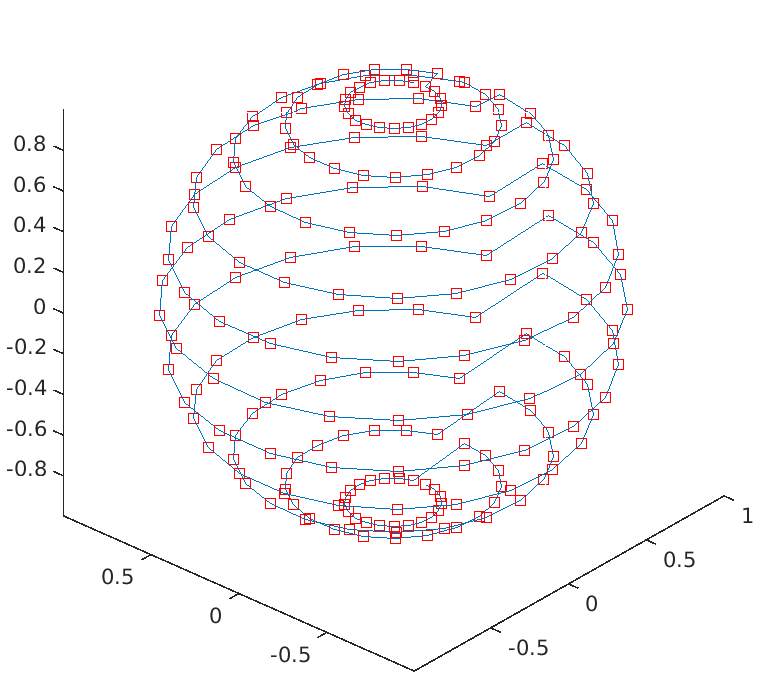
\includegraphics[height=0.4\textheight]{sphere}
  \caption{Représentation de la sphère pour $L=10$.}
  \label{fig:sph}
\end{figure}

Ce genre de quadrature se génère avec une complexité en $I \times J^2 \approx \mathcal{O}(L^3)$. Le terme en $J^2$ se justifie par la
recherche des valeurs propres pour calculer les points et les poids. Dans la suite, nous allons faire quelques vérifications sur les
harmoniques sphériques
\[
  Y_{lm}(\hs) = \sqrt{\frac{(2l+1)(l-m)!}{4\pi(l+m)!}} P^m_l(\cos(\theta)) e^{im\varphi} \quad \forall l \geq 0,~ \forall -l \leq m \leq l
\]
dont on connaît la formule d'intégration théorique
\[
  \int_{S^2} Y_{lm} = \sum_{i,j} w^\varphi_i w^\theta_j Y_{lm}(\theta_j, \varphi_i) = \quad
  \begin{cases}
    2\sqrt{\pi} & \text{si } l=m=0 \\
    0 & \text{sinon.}
  \end{cases}
\]
On obtient en effet les valeurs attendues avec des nombres complexes dont la norme est d'environs $10^{-16}$ pour les valeurs non nulles de
$l, m$ et est proche de $2\sqrt{\pi}$ pour $(l, m) = (0,0)$ à la précision flottante près.

Cependant, on aimerait en savoir plus sur comment se comporte la valeur de cette intégrale en fonction du $L$. On observé qualitativement dans
un premier temps que pour un $l$ fixé et pour tout $m\in[0,l]$, il y a une valeur seuil de
$L$ à partir de laquelle la valeur de l'intégrale chute de plusieurs ordres de grandeur en passant de l'unité à $10^{-16}$. La dépendance
de ce $L_{\smbox{seuil}}$ par rapport au paramètre $l$ est tracée en \autoref{fig:L_min_l}, o\`u on peut supposer une relation
linéaire avec un coefficient d'environ $1/2$, c'est donc bien la loi des $l<2L$ que l'on retrouve. 
\begin{figure}
  \centering
  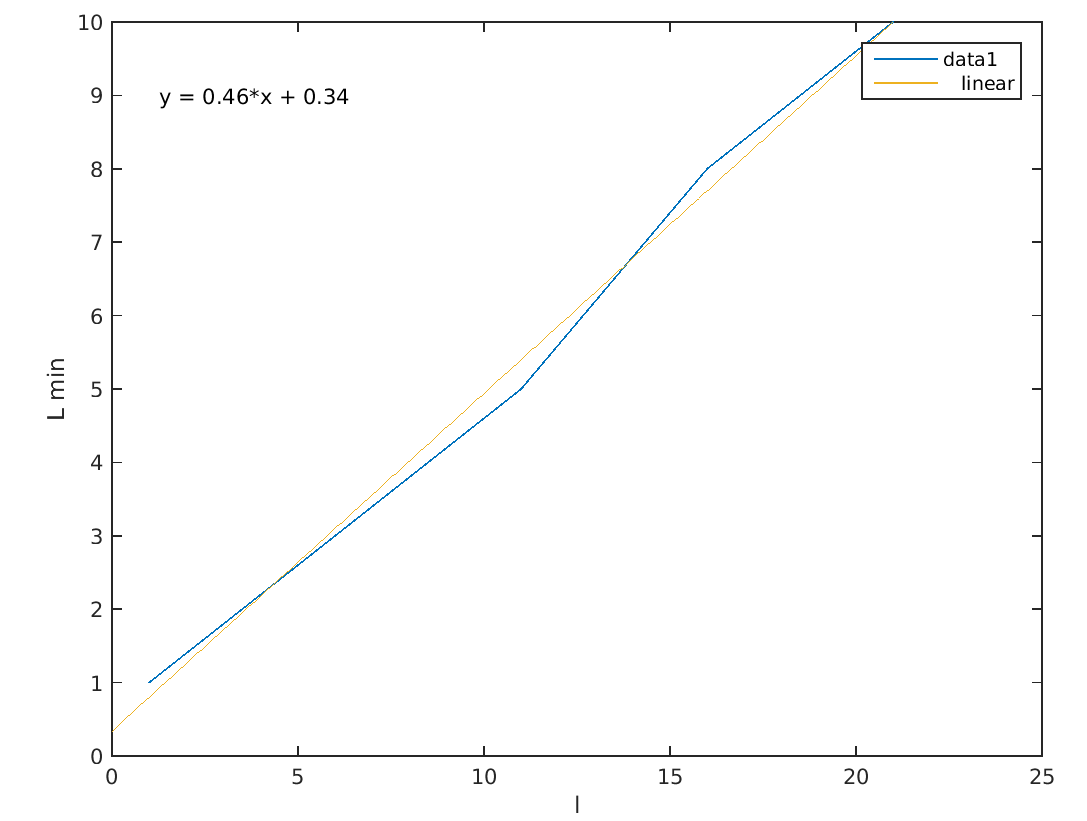
\includegraphics[height=0.4\textheight]{L_min_l}
  \caption{Valeur de $L_{\smbox{seuil}}$  à partir de laquelle l'intégrale est supposée juste en fonction de $l$.}
  \label{fig:L_min_l}
\end{figure}

On ne s'attend pas à avoir un comportement identique plus tard mais on peut espérer trouver des similarités du fait de la présence de
polynômes de Legendre dans les deux cas, sinon cette étude nous aura au moins permis de savoir de quel ordre de grandeur on doit choisir $L$
pour des cas simples.

\begin{rmq}
  Suite aux bugs décrits plus loin, d'autres tests ont été menés avec d'autres fonctions d'intégration :
  \begin{align*}
    f_x : &\R^3 \to \R \\
          &(x, y, z) \to x
  \end{align*}
  \begin{align*}
    f_y : &\R^3 \to \R \\
          &(x, y, z) \to y
  \end{align*}                   
  \begin{align*}
    f_z : &\R^3 \to \R \\
          &(x, y, z) \to z
  \end{align*}
  qui sont toutes d'intégrale théoriquement nulle. C'est en effet le cas numériquement, ce qui confirme notre quadrature. 
\end{rmq}

\section{Éléments de calculs de la fonction $\lG_L$}

\begin{rmq}
  Dans la suite on note $\circ$ le produit terme à terme (aussi appelé produit de Schur).
\end{rmq}

On rappelle que les fonctions Hankel sphériques $h^{(1)}_n$ s'obtiennent à partir des fonctions de Hankel $H^{(1)}_n$ cartésiennes
implémentées dans MATLAB avec la formule
\[
  h^{(1)}_n(z) = \sqrt{\frac{\pi}{2z}}H^{(1)}_{n+1/2}(z), \quad \forall z \in \C, \forall n \in \N
\]
Le calcul de $G_L$ se fait en trois étapes indépendantes qui peuvent séparées dans un but d'optimisation bien que l'ordre soit fixé
\begin{enumerate}
\item Calcul des points de la quadrature ;
\item Calcul de la fonction $\lG_L$ ;
\item Calcul des exponentielles complexes et de l'intégrale.
\end{enumerate}
Le calcul vectorialisé de la valeur de $\lG_L(\hs, r_0)$ avec $N_{\hs}$ points de quadrature se fait comme suit
\begin{enumerate}
\item Créer le vecteur $F\in\C^L$ tel que $F_p = (2p+1) i^p, \forall 1\leq p \leq L $ 
\item Créer le vecteur $H\in\C^L$ tel que $H_p = h^{(1)}_p(k|r_0|)$
\item Calculer le vecteur $K\in\C^L$ tel que $K = \frac{i k}{16 \pi^2}\,F \circ H$
\item Créer la matrice $\mathbb{P}\in\mathcal{M}_{N_{\hs}\times L}(\C)$ telle que $\mathbb{P}_{sp} = P_p(\cos(\hs_s, r_0))$
\item Calculer le vecteur $G\in\C^{N_{\hs}}$ tel que $G = \mathbb{P}K$.
\end{enumerate}
Le vecteur $G$ est le résultat vectorialisé pour les tous les points de la sphère : $G_s = \lG_L(\hs_s, r_0), ~ \forall s<N_{\hs}$.


Pour vérifier que cette fonction donne de bons résultats, on les compare avec ceux de $G(r)$ pour plusieurs paramètrisations de $L,~ r_0$
et $k$. Pour cela on fixe un $r_0$ relativement grand. On pose ensuite un ensemble de $N_x$ (\emph{resp. $N_y$}) points aléatoires dans une boule de rayon $d_x$
(\emph{resp. $d_y$}) tel que $\max(d_x, d_y) \ll |r_0|$. On fixe ensuite $k$ tel que

\begin{equation}
  \label{eq:cddk}
  k\geq 0.3\cdot 2 \pi/ |r_0| \approx 2.1/|r_0|.
\end{equation}


\emph{\small Cependant... Malgré une bonne dizaine d'heures de recherche, impossible de débugger la fonction qui calcule $\lG_L$... Les résultats, bien
que du bon ordre de grandeur ne sont pas continus en $r_0$ dans la majorités des cas o\`u l'on s'attendrait à avoir une décroissance en
$1/|r_0|$. On ne retrouve pas non plus de forme en $\sin(x)$ ou $\cos(x)$ sur les parties réelles et imaginaires comme on pourrait
l'espérer.} Voici ce que j'aurais écrit si le code ne s'était pas mis à marcher à 22h la veille de rendre le rapport... Moyennant ``bricolage'' (coefficient -1...) on
retrouve maintenant de bons résultats.

Dans la \autoref{fig:err_L} on voit l'erreur calculée comme la norme de Foebus de la différences entres les matrices obtenues par méthodes
directe et par méthode du kernel :
\[
  err = \sum_{ij} (\Gm_{ij} - (\Gm_L)_{ij})^2.
\]
On voit que celle ci chute plus vite que polynomialement. On s'intéresse en \autoref{fig:err_x0} à la même erreur commise en fonction de $|r_0|$
à $k$ constant. On voit encore une fois une décroissance très forte puisqu'elle semble exponentielle alors que le graphe est en semi log. Les
petits sauts d'erreurs pouvant être dûs au tirage aléatoire des points $x$ pour chaque valeur de $x_0$. Enfin en \autoref{fig:tps_npts} on
observe le temps de calcul en fonction du nombre de points $N_x = N_y = N$. On voit que malgré une grosse ordonnée à l'origine, la courbe de
temps de la méthode kernel devient rentable pour $N$ grand. Ce phénomène est amplifié par le fait que les demandes en ressources
aux environs de $10^4$ points explosent et font passer une partie des données sur la mémoire \texttt{swap} ce qui augmente énormément les temps de calcul.

\begin{figure}
  \centering
  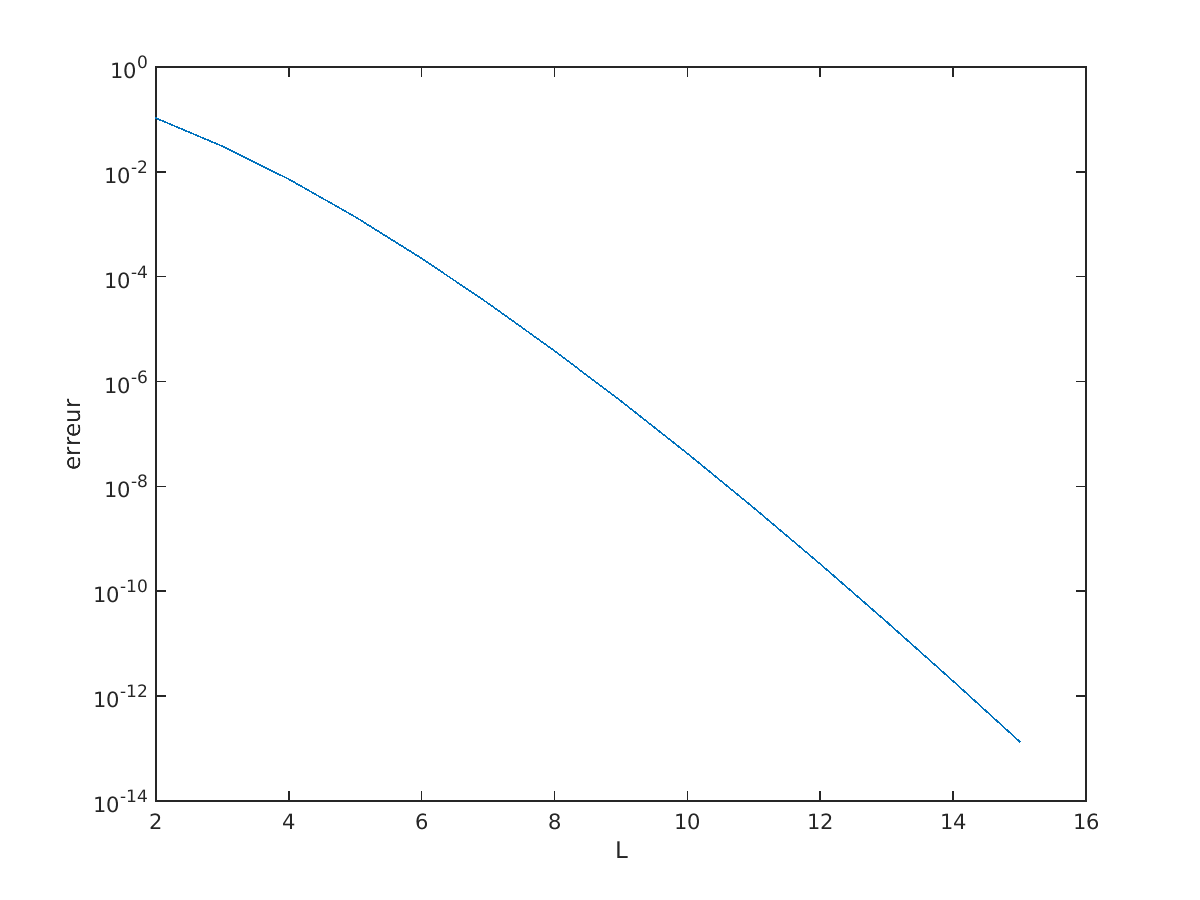
\includegraphics[height=.35\textheight]{err_L}
  \caption{Erreur en fonction de $L$. On a ici $k=2,~x_0=(10,0,0),~y_0=(1,0,0),~ N_x = N_y = 50, ~d_x=d_y=1.$}
  \label{fig:err_L}
\end{figure}

\begin{figure}
  \centering
  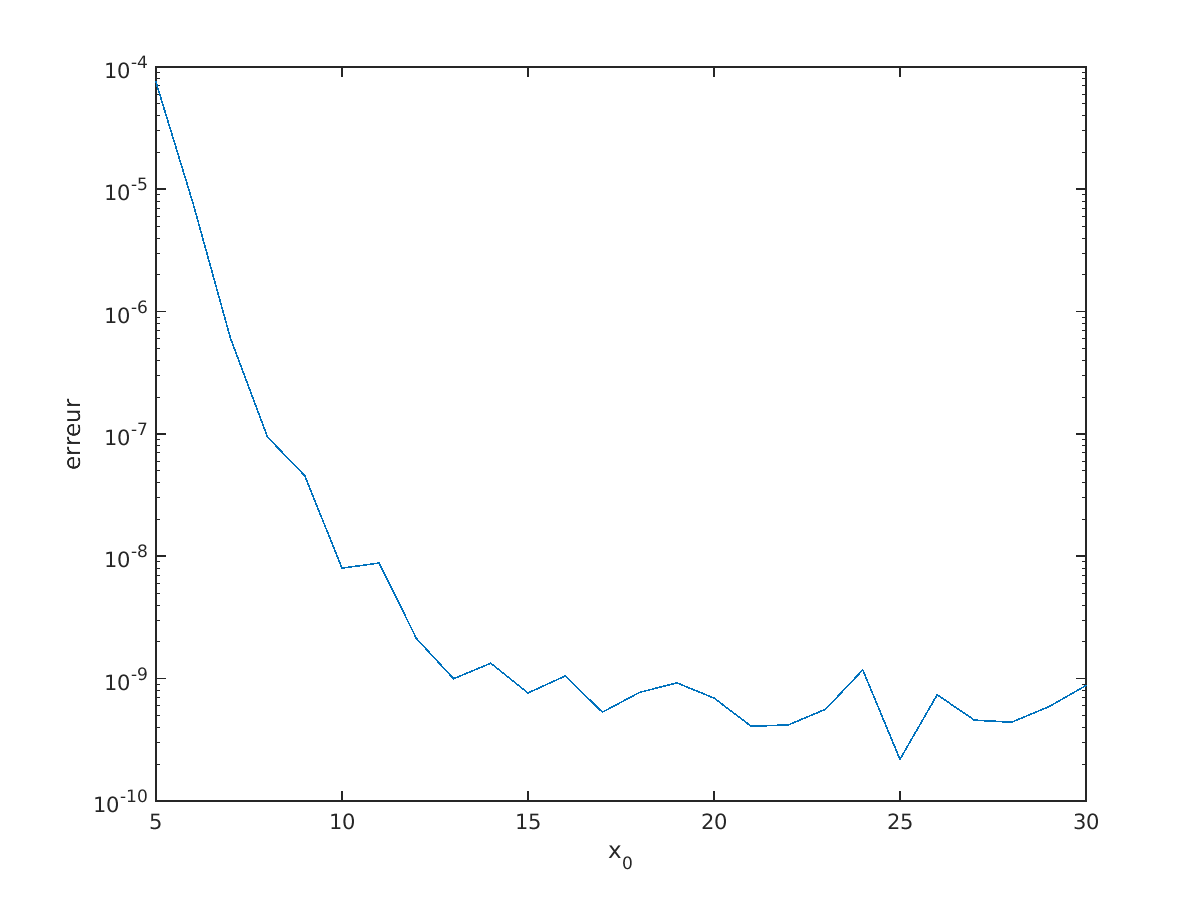
\includegraphics[height=.35\textheight]{err_x0}
  \caption{Erreur en fonction de $|r_0|$. On a ici $k=2,~L=12,~y_0=(1,0,0),~ N_x = N_y = 50, ~d_x=d_y=1.$}
  \label{fig:err_x0}
\end{figure}

\begin{figure}
  \centering
  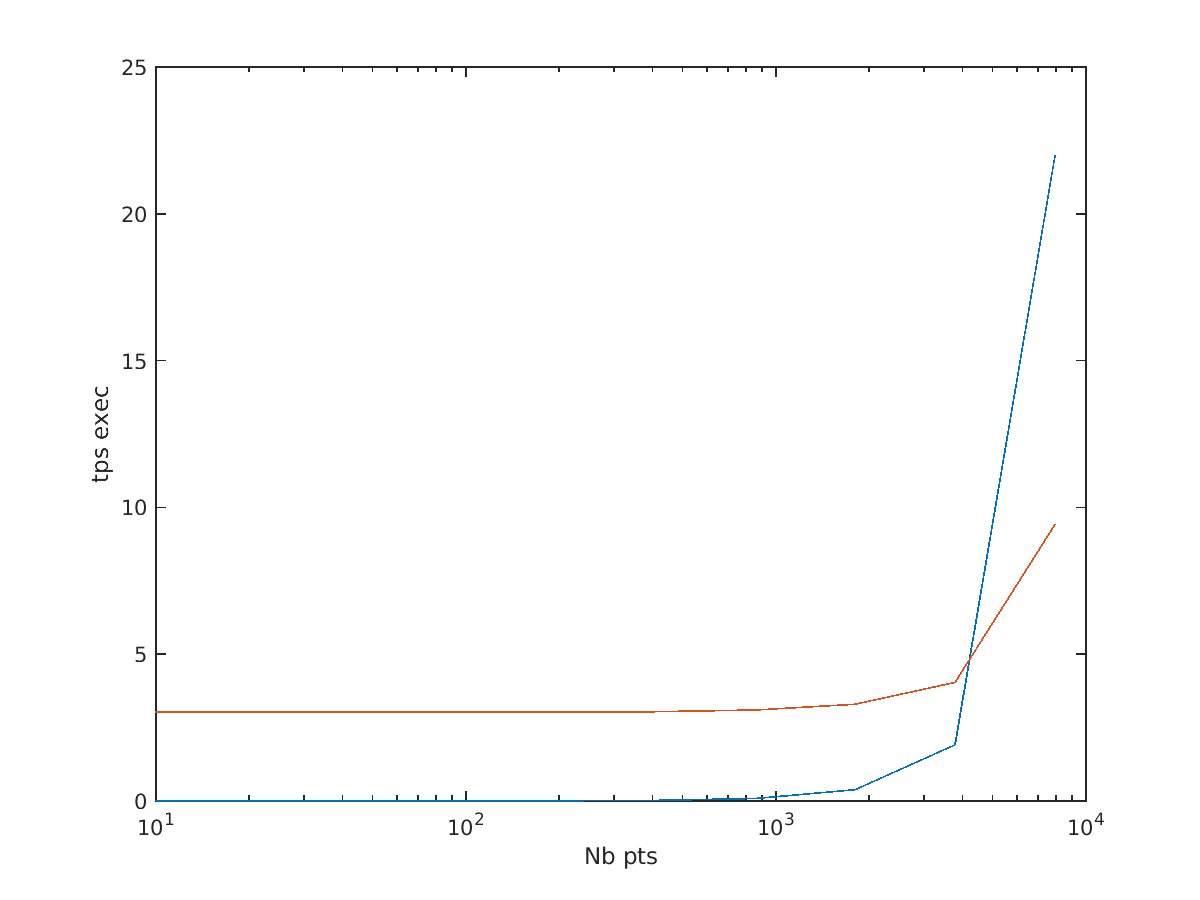
\includegraphics[height=.35\textheight]{tps_npts}
  \caption{Temps de calcul en fonction de $N_x = N_y = N$. On a ici $k=1,~L=12,~x_0=(10,0,0),~y_0=(1,0,0), ~d_x=d_y=1$. En rouge on voit la
    courbe pour la méthode kernel, en bleu la méthode classique. Les temps sont donnés en secondes.}
  \label{fig:tps_npts}
\end{figure}


\section{Découpage du maillage en boîtes adaptées}

Il s'agit maintenant de faire un partitionnement du maillage de la sphère qui soit cohérent avec les approximations. Pour cela on a récupéré
sur le net un objet MATLAB nommé
\texttt{OcTree}\footnote{\href{https://fr.mathworks.com/matlabcentral/fileexchange/40732-octree-partitioning-3d-points-into-spatial-subvolumes}{Le
  lien vers la source. }}
ou les routines de bases pour partitionner sont codées. Parmi les paramètres à fixer on choisie d'empêcher plus de 2 niveaux de profondeurs
dans l'arbre. De plus on donne une taille minimale aux cubes en fonction de $k$ avec la règle énoncée en \autoref{eq:cddk}. 
\begin{rmq}
  On ne travaillera qu'au niveau feuille, mais les niveaux 0 et 1 étant particuliers il faut monter au niveau 2 de profondeur
  pour que l'algorithme de partionnement fonctionne correctement.
\end{rmq}

Une fois qu'on a filtré les cubes de sorte à n'avoir que les feuilles de l'arbre, il faut ajouter une méthode pour sauvegarder les
voisinages, puisque les méthodes de kernel ne sont applicables que dans les partitions lointaines \ie à plus d'un cube de distance.
On ne peut en effet pas appliquer la méthode kernel sur les cubes voisins car pour un point de notre partition à la frontière avec
la boîte voisine, les points de la seconde sont bien trop proches pour que la méthode kernel soit adaptée. On code cette information sous la
forme d'une matrice symétrique $\mathbb{V} \in \mathcal{M}_{N_{\smbox{p}}}(\{0,1\})$ telle que
\[
  \mathbb{V}_{ij} =
  \begin{cases}
    1 &  \text{si les boîtes $i$ et $j$ sont voisines ou bien si } i=j \\
    0 & \text{sinon}.
  \end{cases}
\]

On peut voir un de ces découpages dans la \autoref{fig:part}, qui semble coloré néanmoins complexe. 

\begin{figure}
  \centering
  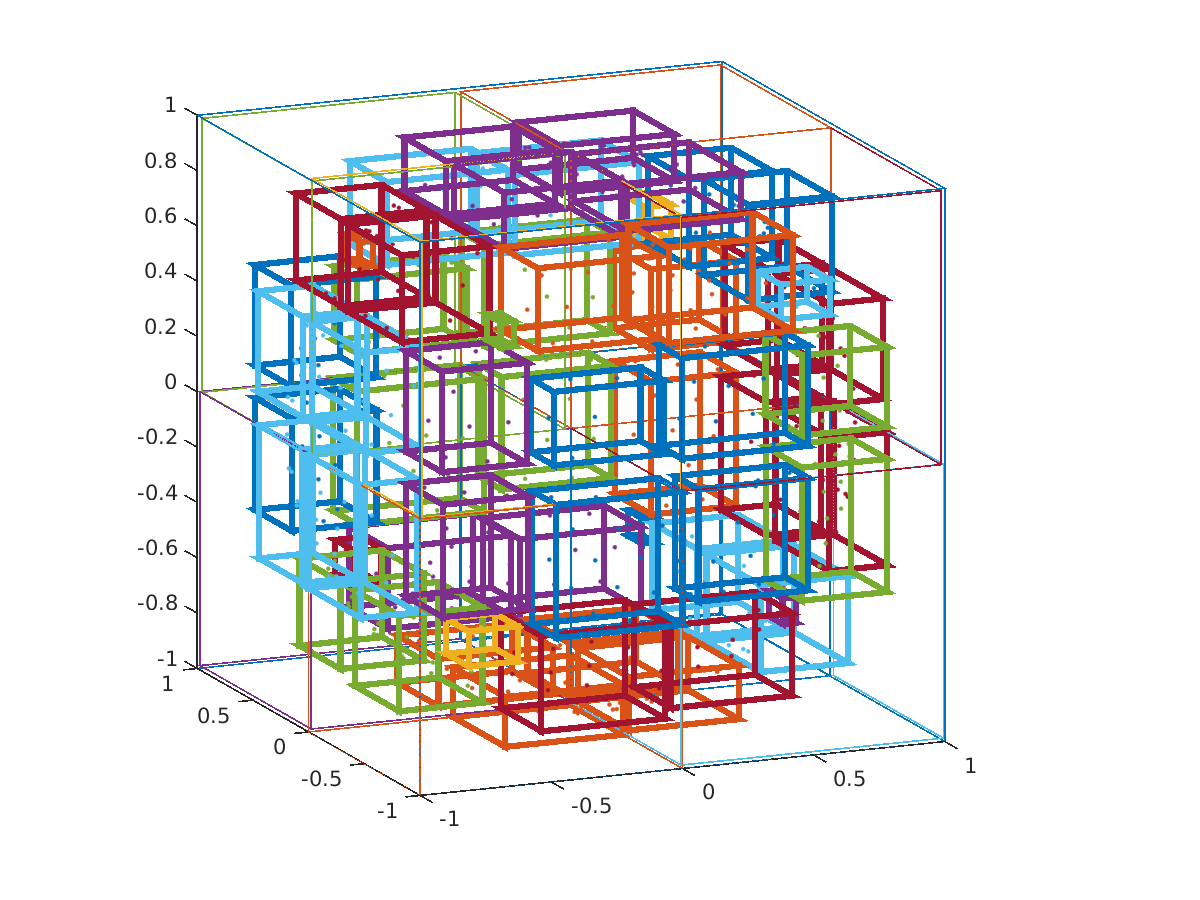
\includegraphics[height=0.35\textheight]{partsph}
  \caption{Découpage de la sphère}
  \label{fig:part}
\end{figure}

La routine principale pour faire la FMM est cependant buggée et je n'ai plus le temps de corriger les problèmes...

\appendix

\section{Description des fonctions }


\begin{table}
  \centering
  \begin{tabular}{|c|p{.7\textwidth}|}
    \hline
    Fonction                      & Description                                                                              \\ 
    \hline \hline
    \texttt{besselh\_Sph.m    }   & Calcul des fonctions de Hankel sphériques à partir des fonctions de Hankel cartésiennes. \\
    \hline
    \texttt{calc\_quad.m      }   & Calcul des points et des poids de la quadrature nécessaire.                              \\
    \hline
    \texttt{dist.m           }    & Calcul la distance point à point entre deux vecteurs (renvoie donc une matrice).         \\
    \hline
    \texttt{FMM\_G.m          }   & Fait le nécessaire pour le calcul de \autoref{eq:goal} par la méthode la FMM. Construction de l'arbre, recherche des
                                 voisins, calcul de la quadrature, calcul des valeurs de $G_L$ locales et produits. Pas tout à fait finie
                                 pour être honnête, $\rho$ n'apparaît pas dans cette version, on construit donc actuellement l'ensemble de la
                                 matrice...                                                                                 \\
    \hline
    \texttt{G\_devel\_G\_L.m    } & Calcul $\lG_L$ pour $L,~k,$ et une quadrature données.                                   \\
    \hline
    \texttt{G\_devel.m        }   & Calcul de $G_L$ avec $\lG_L$ et une quadrature données.                                  \\
    \hline
    \texttt{G.m              }    & Calcul classique de la matrice $\Gm$.                                                    \\
    \hline
    \texttt{integ\_SphHarmo.m }   & Calcul de l'intégrale d'une harmonique sphérique.                                        \\
    \hline
    \texttt{main.m           }    & Ensemble des scripts de plot présentés dans ce rapport.                                  \\
    \hline
    \texttt{OcTree.m         }    & Objet MATLAB qui permet le découpage spatial de la sphère.                               \\
    \hline
    \texttt{read\_meshfile.m  }   & Méthode pour lire un fichier msh.                                                        \\
    \hline
  \end{tabular}
  \caption{Description des fonctions utilisées.}
  \label{tab:funcs}
\end{table}



\end{document}       
%%% Local Variables: 
%%% mode: latex      
%%% TeX-master: t    
%%% End:             